\section{Methodology}

%\subsection{分栏显示}
\subsection{From R-CNN to YOLO}
\begin{frame}{R-CNN Series}
    \begin{columns}
        \begin{column}{0.5\textwidth}
            R-CNN is an object detection model that uses selective search for region proposals, feeds these into a pre-trained CNN for feature extraction, and then classifies and refines the regions using SVMs and bounding box regressors. \\
            \bigskip
            It laid the foundation for deep learning-based object detection but was computationally intensive.

        \end{column}
        \begin{column}{0.5\textwidth}
            \begin{figure}[h]
                \centering
                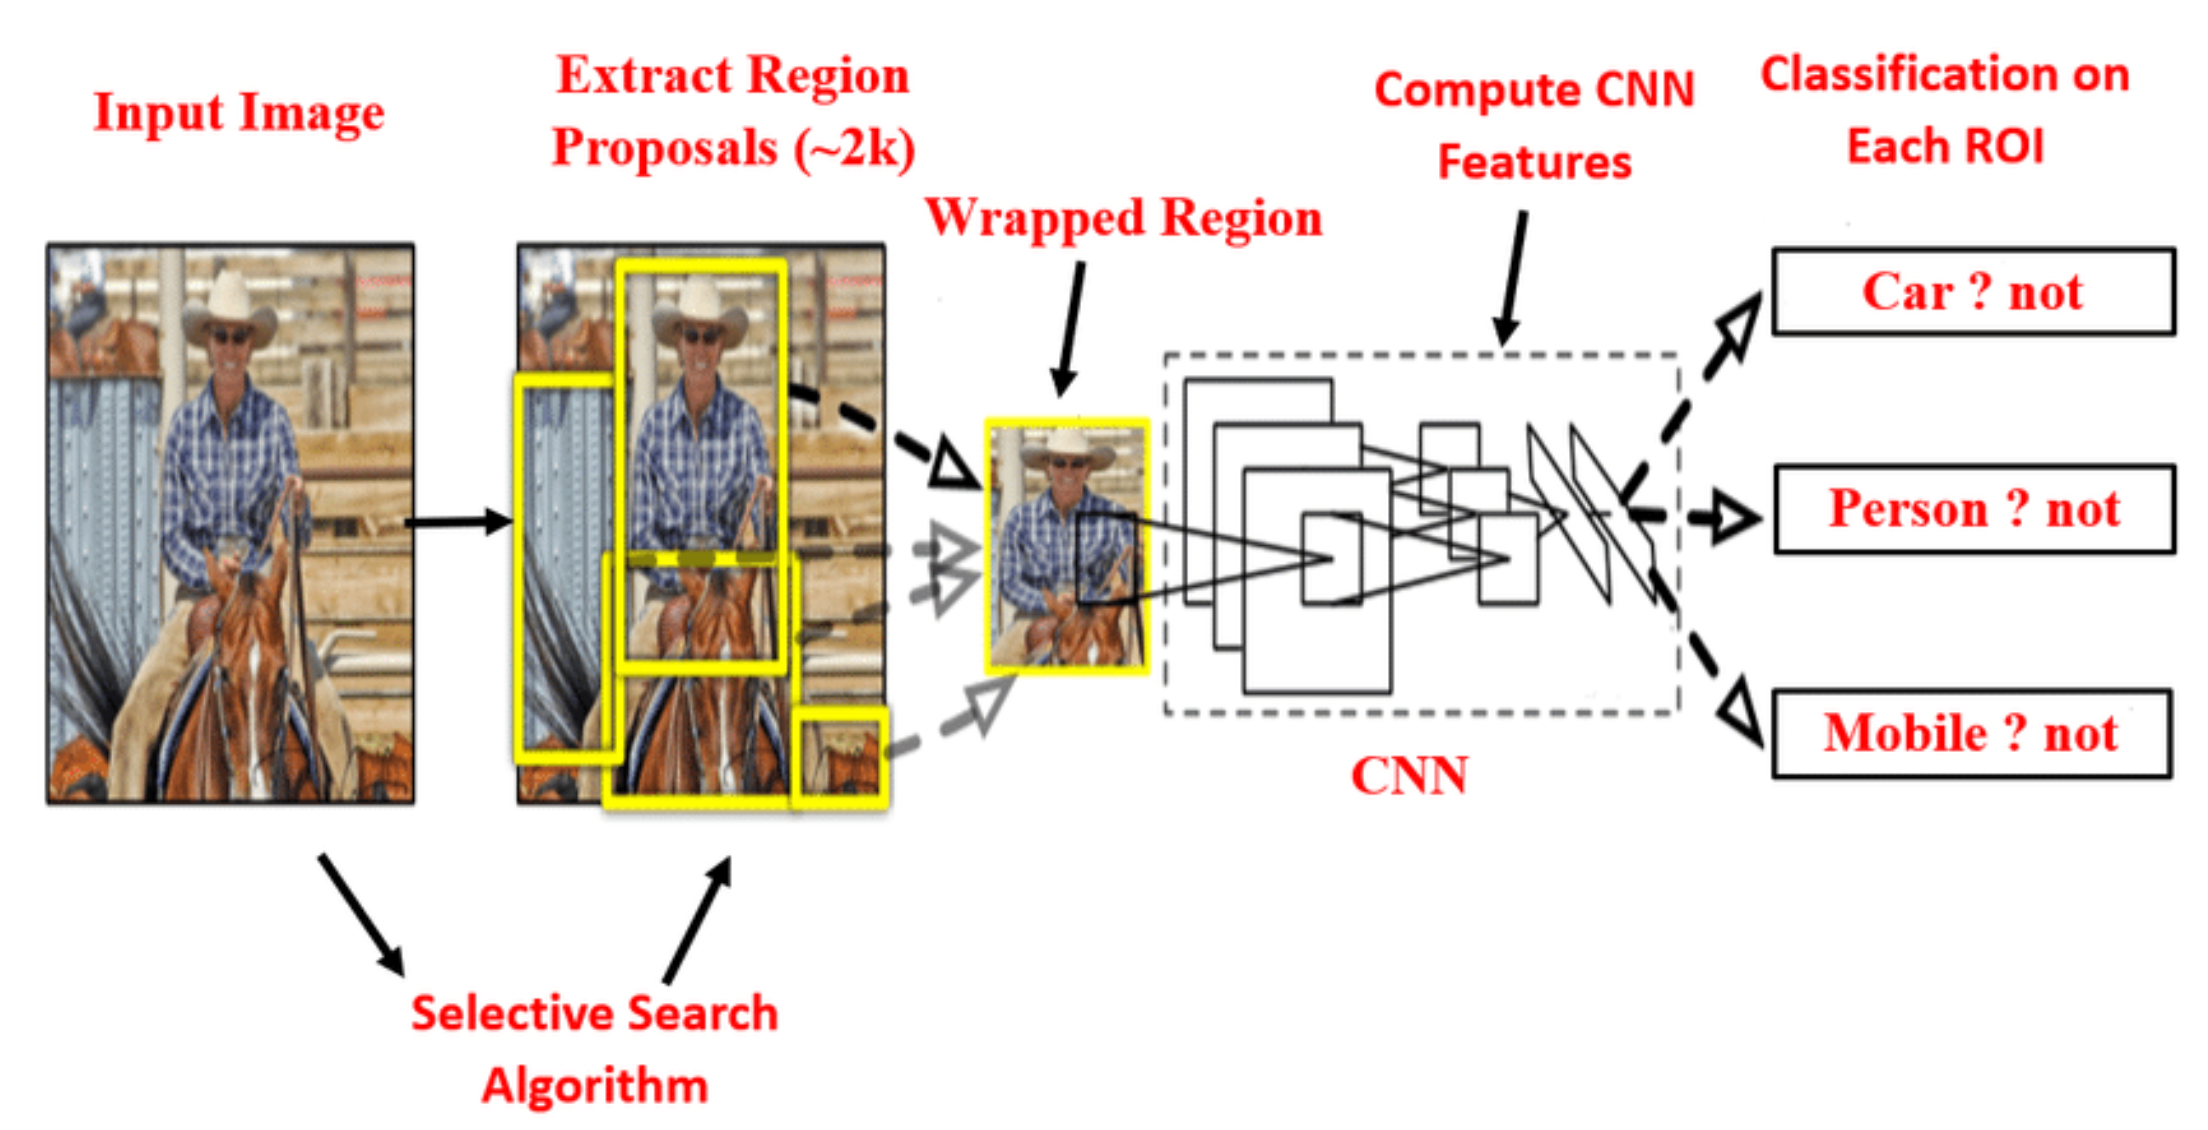
\includegraphics[width=\textwidth]{images/rcnn.png}
                \caption{R-CNN}
                \label{fig:rcnn}
            \end{figure}
        \end{column}
    \end{columns}
\end{frame}

\begin{frame}{R-CNN series}
	\begin{columns}
		\begin{column}{0.5\textwidth}
			\begin{figure}[h]
				\centering
				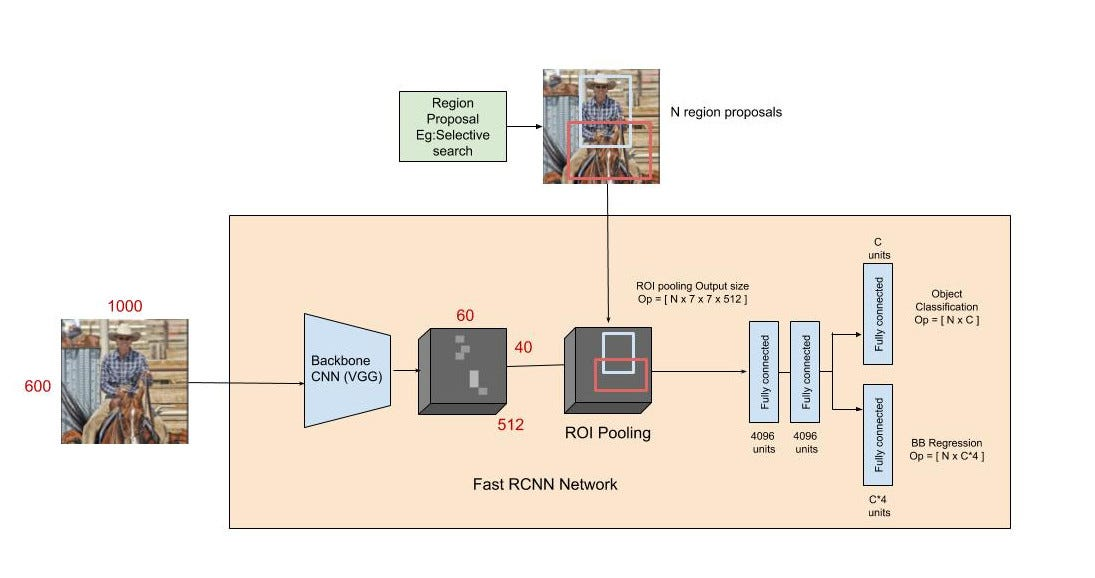
\includegraphics[width=\textwidth]{images/fast-rcnn.jpeg}
				\caption{Fast R-CNN}
				\label{fig:fast-rcnn}
			\end{figure}
		\end{column}
		\begin{column}{0.5\textwidth}
			\begin{figure}[h]
				\centering
				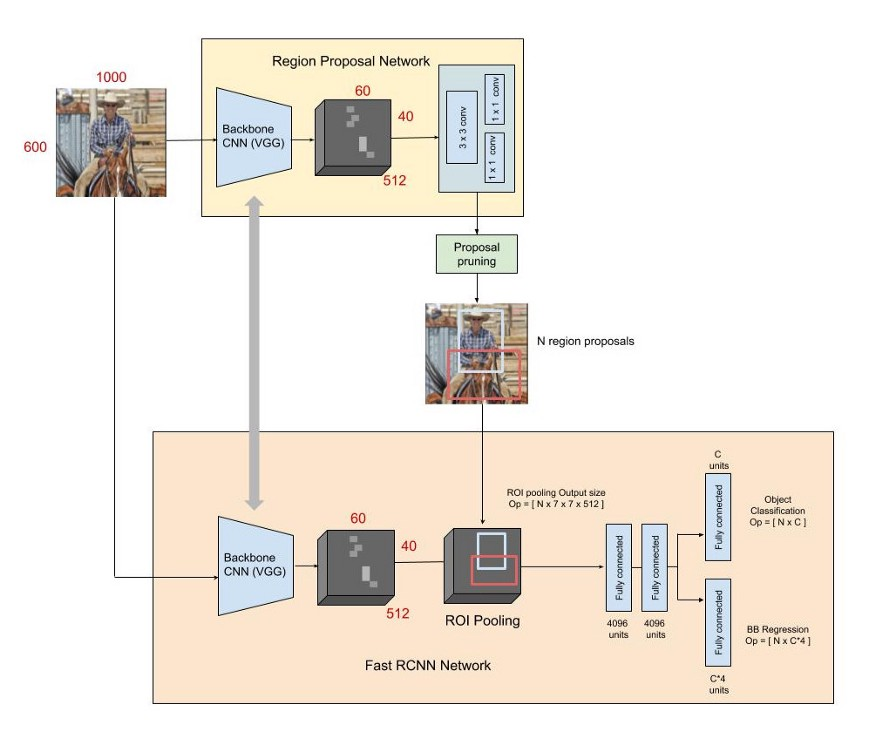
\includegraphics[width=\textwidth]{images/faster-rcnn.jpeg}
				\caption{Faster R-CNN}
				\label{fig:faster-rcnn}
			\end{figure}
		\end{column}
	\end{columns}
\end{frame}

\begin{frame}{You Only Look Once}
	\begin{columns}
		\begin{column}{0.43\textwidth}
			\begin{block}{Innovations}
				\begin{itemize}
				\item Unified detection framework
				\item Real-time detection
				\item Global contextual prediction
				\item Spatially separated bounding boxes
				\item End-to-end training
			\end{itemize}
			\end{block}
		\end{column}
		\begin{column}{0.57\textwidth}
			\begin{figure}[h]
				\centering
				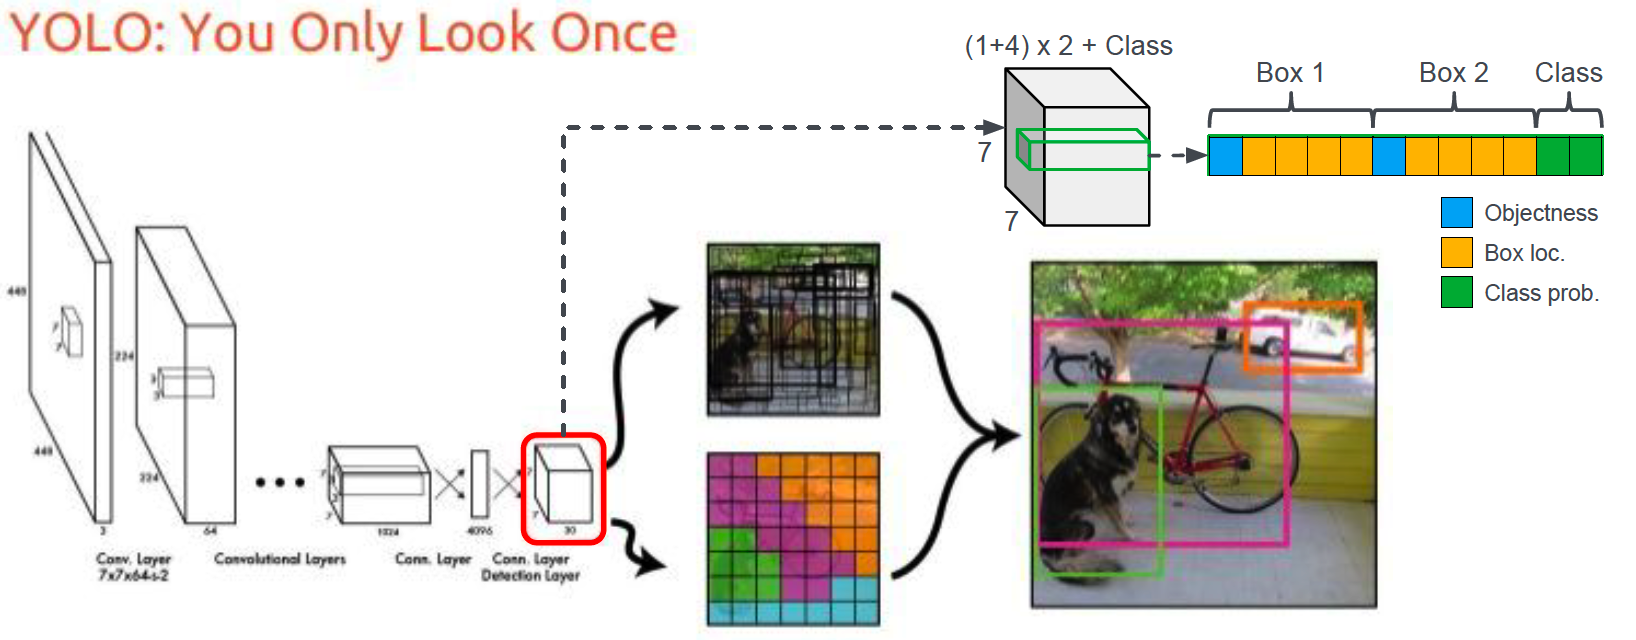
\includegraphics[width=\textwidth]{images/yolov1.png}
				\caption{YOLOv1 architecture}
				\label{fig:yolov1}
			\end{figure}
		\end{column}
	\end{columns}
\end{frame}

\begin{frame}{Loss Function Improvement}
	\begin{block}{YOLOv1}
		\begin{equation}
			\begin{aligned}
				\text { Loss }= & \lambda_{\text {coord }} \sum_{i=0}^{S^2} \sum_{j=0}^B I_{i j}^{\mathrm{obj}}\left[\left(x_i^j-\hat{x}_i^j\right)^2+\left(y_i^j-\hat{y}_i^j\right)^2\right] \\
				& +\lambda_{\text {coord }} \sum_{i=0}^{S^2} \sum_{j=0}^B I_{i j}^{\text {obj }}\left[\left(\sqrt{w_i^j}-\sqrt{\hat{w}_i^j}\right)^2+\left(\sqrt{h_i^j}-\sqrt{\hat{h}_i^j}\right)^2\right] \\
				& +\sum_{i=0}^{s^2} \sum_{j=0}^B I_{i j}^{\text {obj }}\left(C_i^j-\hat{C}_i^j\right)^2 \\
				& +\lambda_{\text {noobj }} \sum_{i=0}^{S^2} \sum_{j=0}^B I_{i j}^{\text {noobj }}\left(C_i^j-\hat{C}_i^j\right)^2 \\
				& +\sum_{i=0}^{s^2} I_{i j}^{\text {obj }} \sum_{c \in \text { classes }}\left(P_i^j(c)-\hat{C}_i^j(c)\right)^2
			\end{aligned}
		\end{equation}
	\end{block}
\end{frame}

\begin{frame}{Loss Function Improvement}
	\begin{block}{YOLOv3}
		\begin{equation}
			\begin{aligned}
				\text { Loss }= & \lambda_{\text {coord }} \sum_{i=0}^{S^2} \sum_{j=0}^B I_{i j}^{\mathrm{obj}}\left[\left(x_i^j-\hat{x}_i^j\right)^2+\left(y_i^j-\hat{y}_i^j\right)^2\right] \\
				& +\lambda_{\text {coord }} \sum_{i=0}^{S^2} \sum_{j=0}^B I_{i j}^{\mathrm{obj}}\left[\left(\sqrt{w_i^j}-\sqrt{\hat{w}_i^j}\right)^2+\left(\sqrt{h_i^j}-\sqrt{\hat{h}_i^j}\right)^2\right] \\
				& -\sum_{i=0}^{s^2} \sum_{j=0}^B I_{i j}^{\mathrm{obj}}\left[\hat{C}_i^j \log \left(C_i^j\right)+\left(1-\hat{C}_i^j\right) \log \left(1-C_i^j\right)\right] \\
				& -\lambda_{\text {noobj }} \sum_{i=0}^{S^2} \sum_{j=0}^B I_{i j}^{\mathrm{noobj}}\left[\hat{C}_i^j \log \left(C_i^j\right)+\left(1-\hat{C}_i^j\right) \log \left(1-C_i^j\right)\right] \\
				& -\sum_{i=0}^{s^2} I_{i j}^{\mathrm{obj}} \sum_{c \in \text { classes }}\left[\hat{P}_i^j \log \left(P_i^j\right)+\left(1-\hat{P}_i^j\right) \log \left(1-P_i^j\right)\right]
			\end{aligned}
		\end{equation}
	\end{block}
\end{frame}

\subsection{The Greatest Works}
\begin{frame}{Masterpieces}
	\begin{columns}
		\begin{column}{0.5\textwidth}
			\begin{figure}[h]
				\centering
				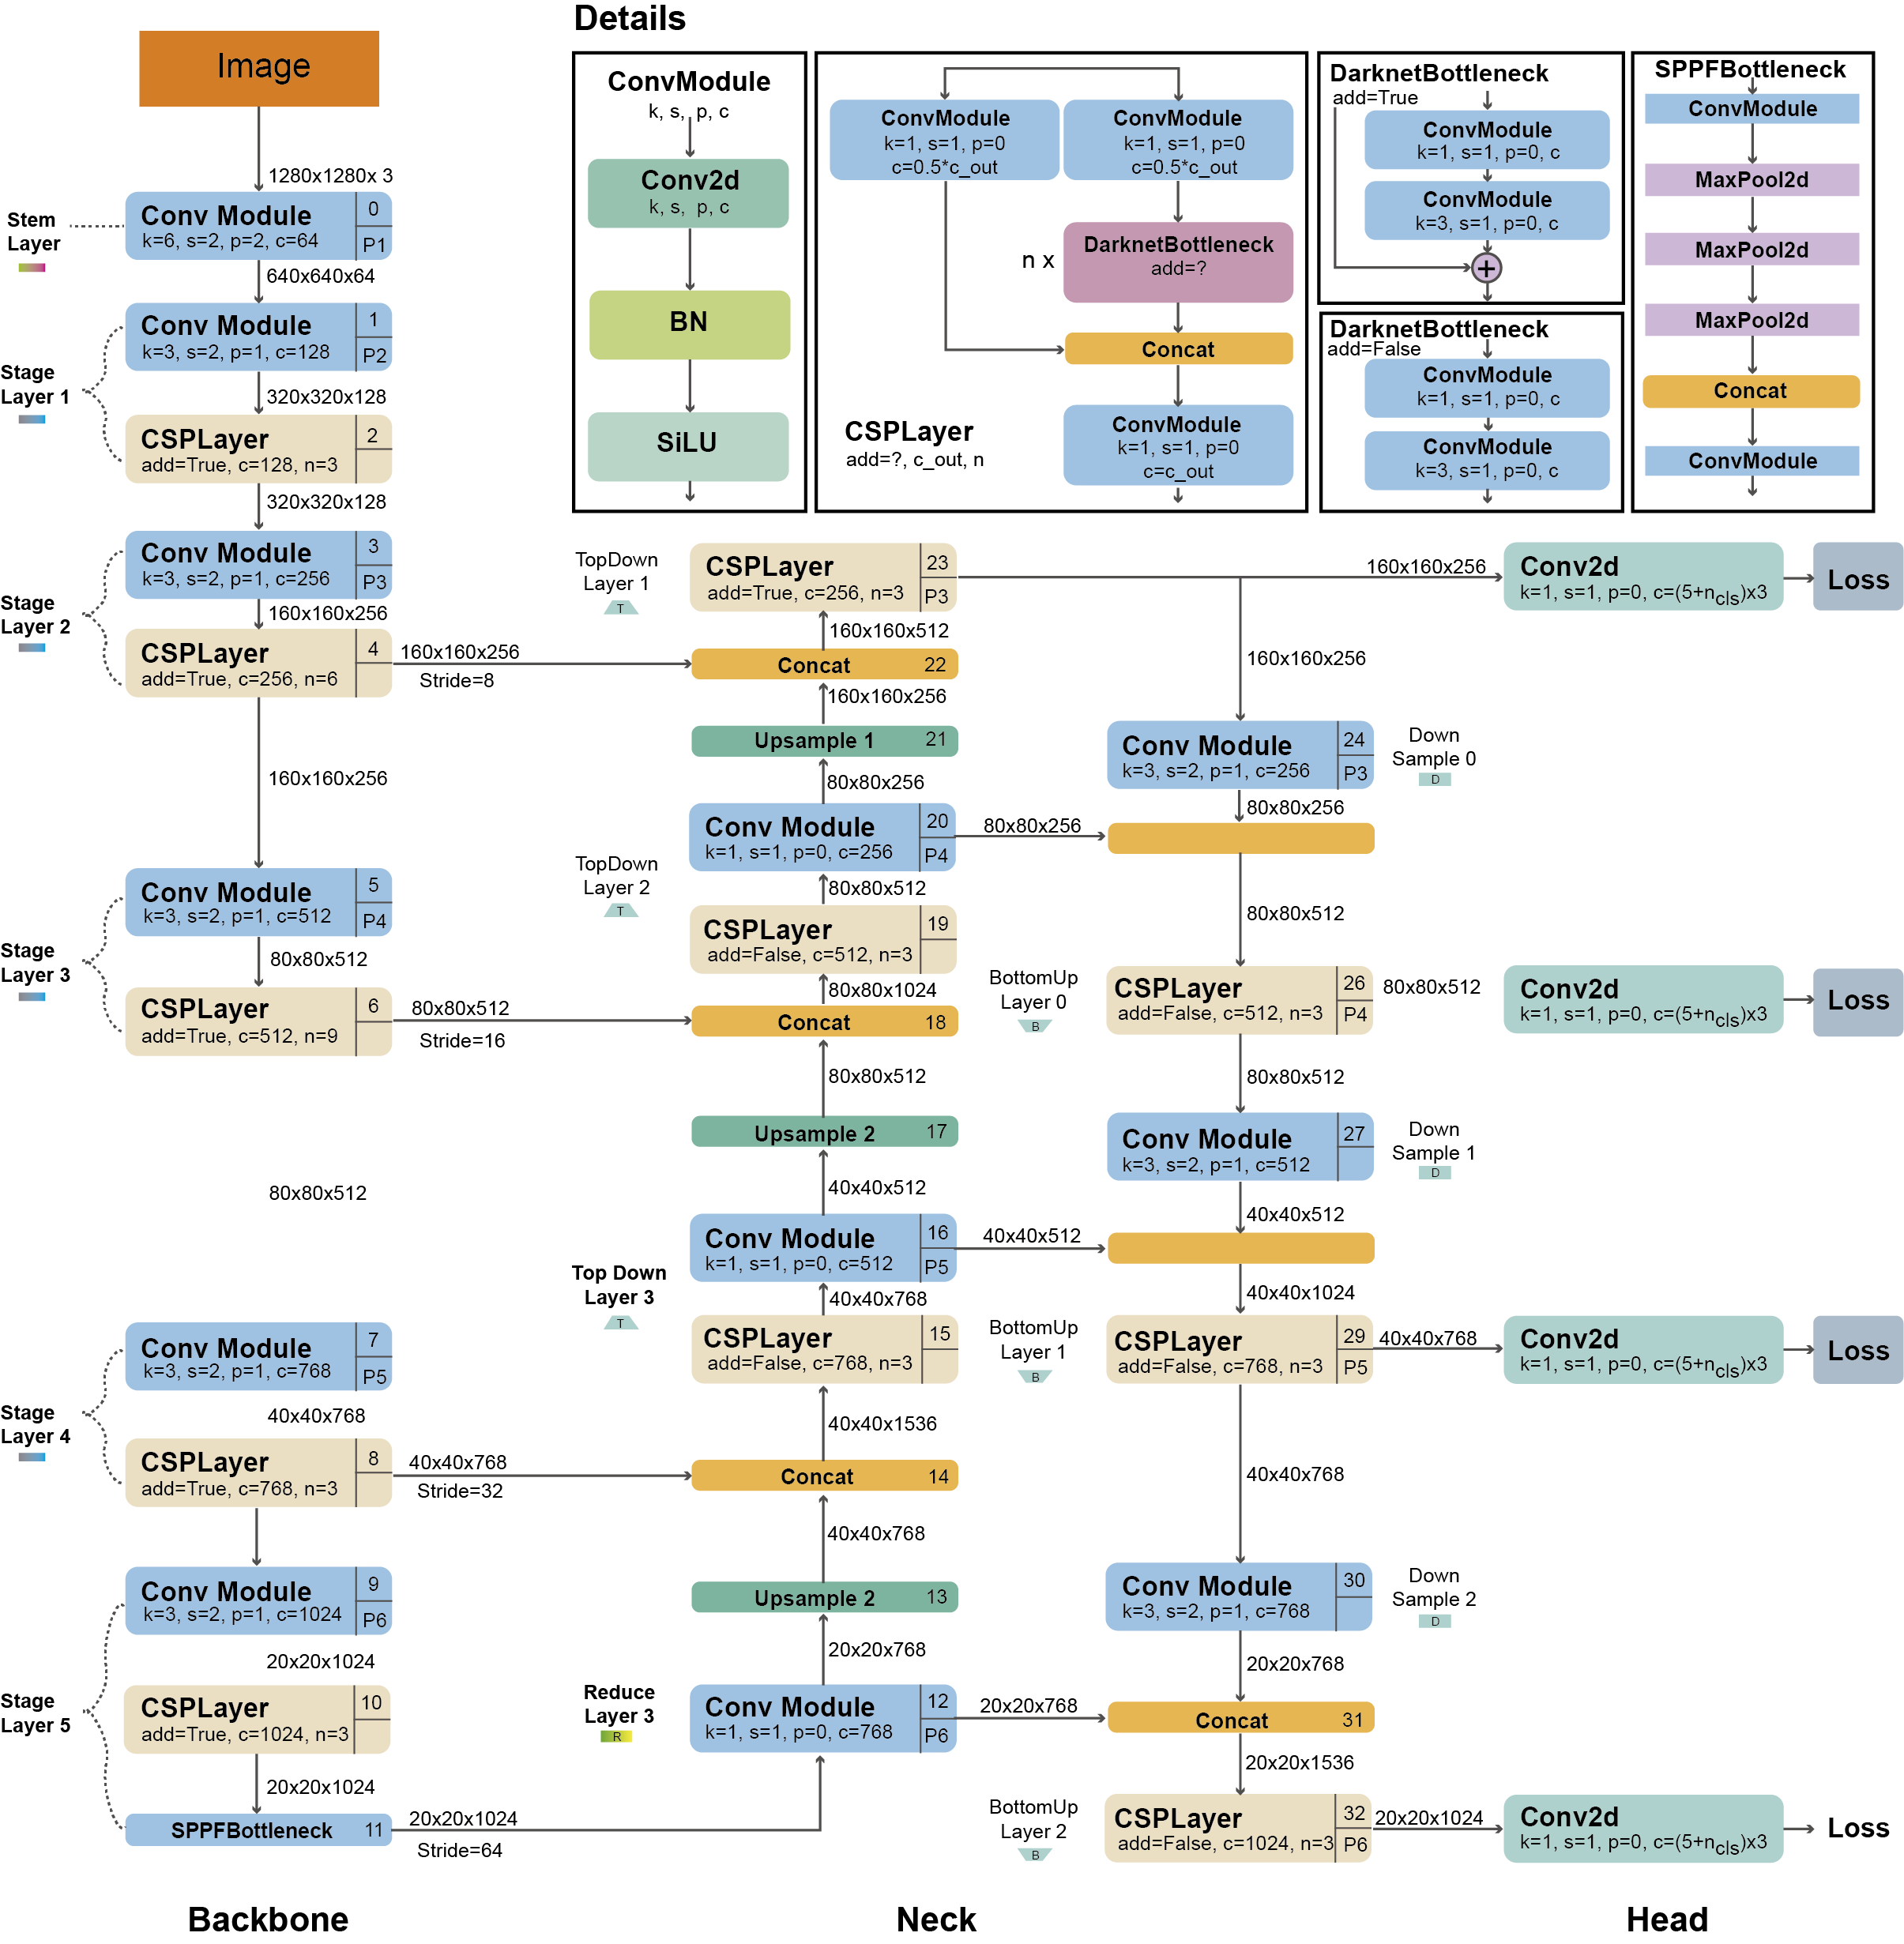
\includegraphics[width=0.88\textwidth]{images/yolov5_architecture.png}
				\caption{YOLOv5 architecture}
				\label{fig:yolov5}
			\end{figure}
		\end{column}
		\begin{column}{0.5\textwidth}
			\begin{figure}[h]
				\centering
				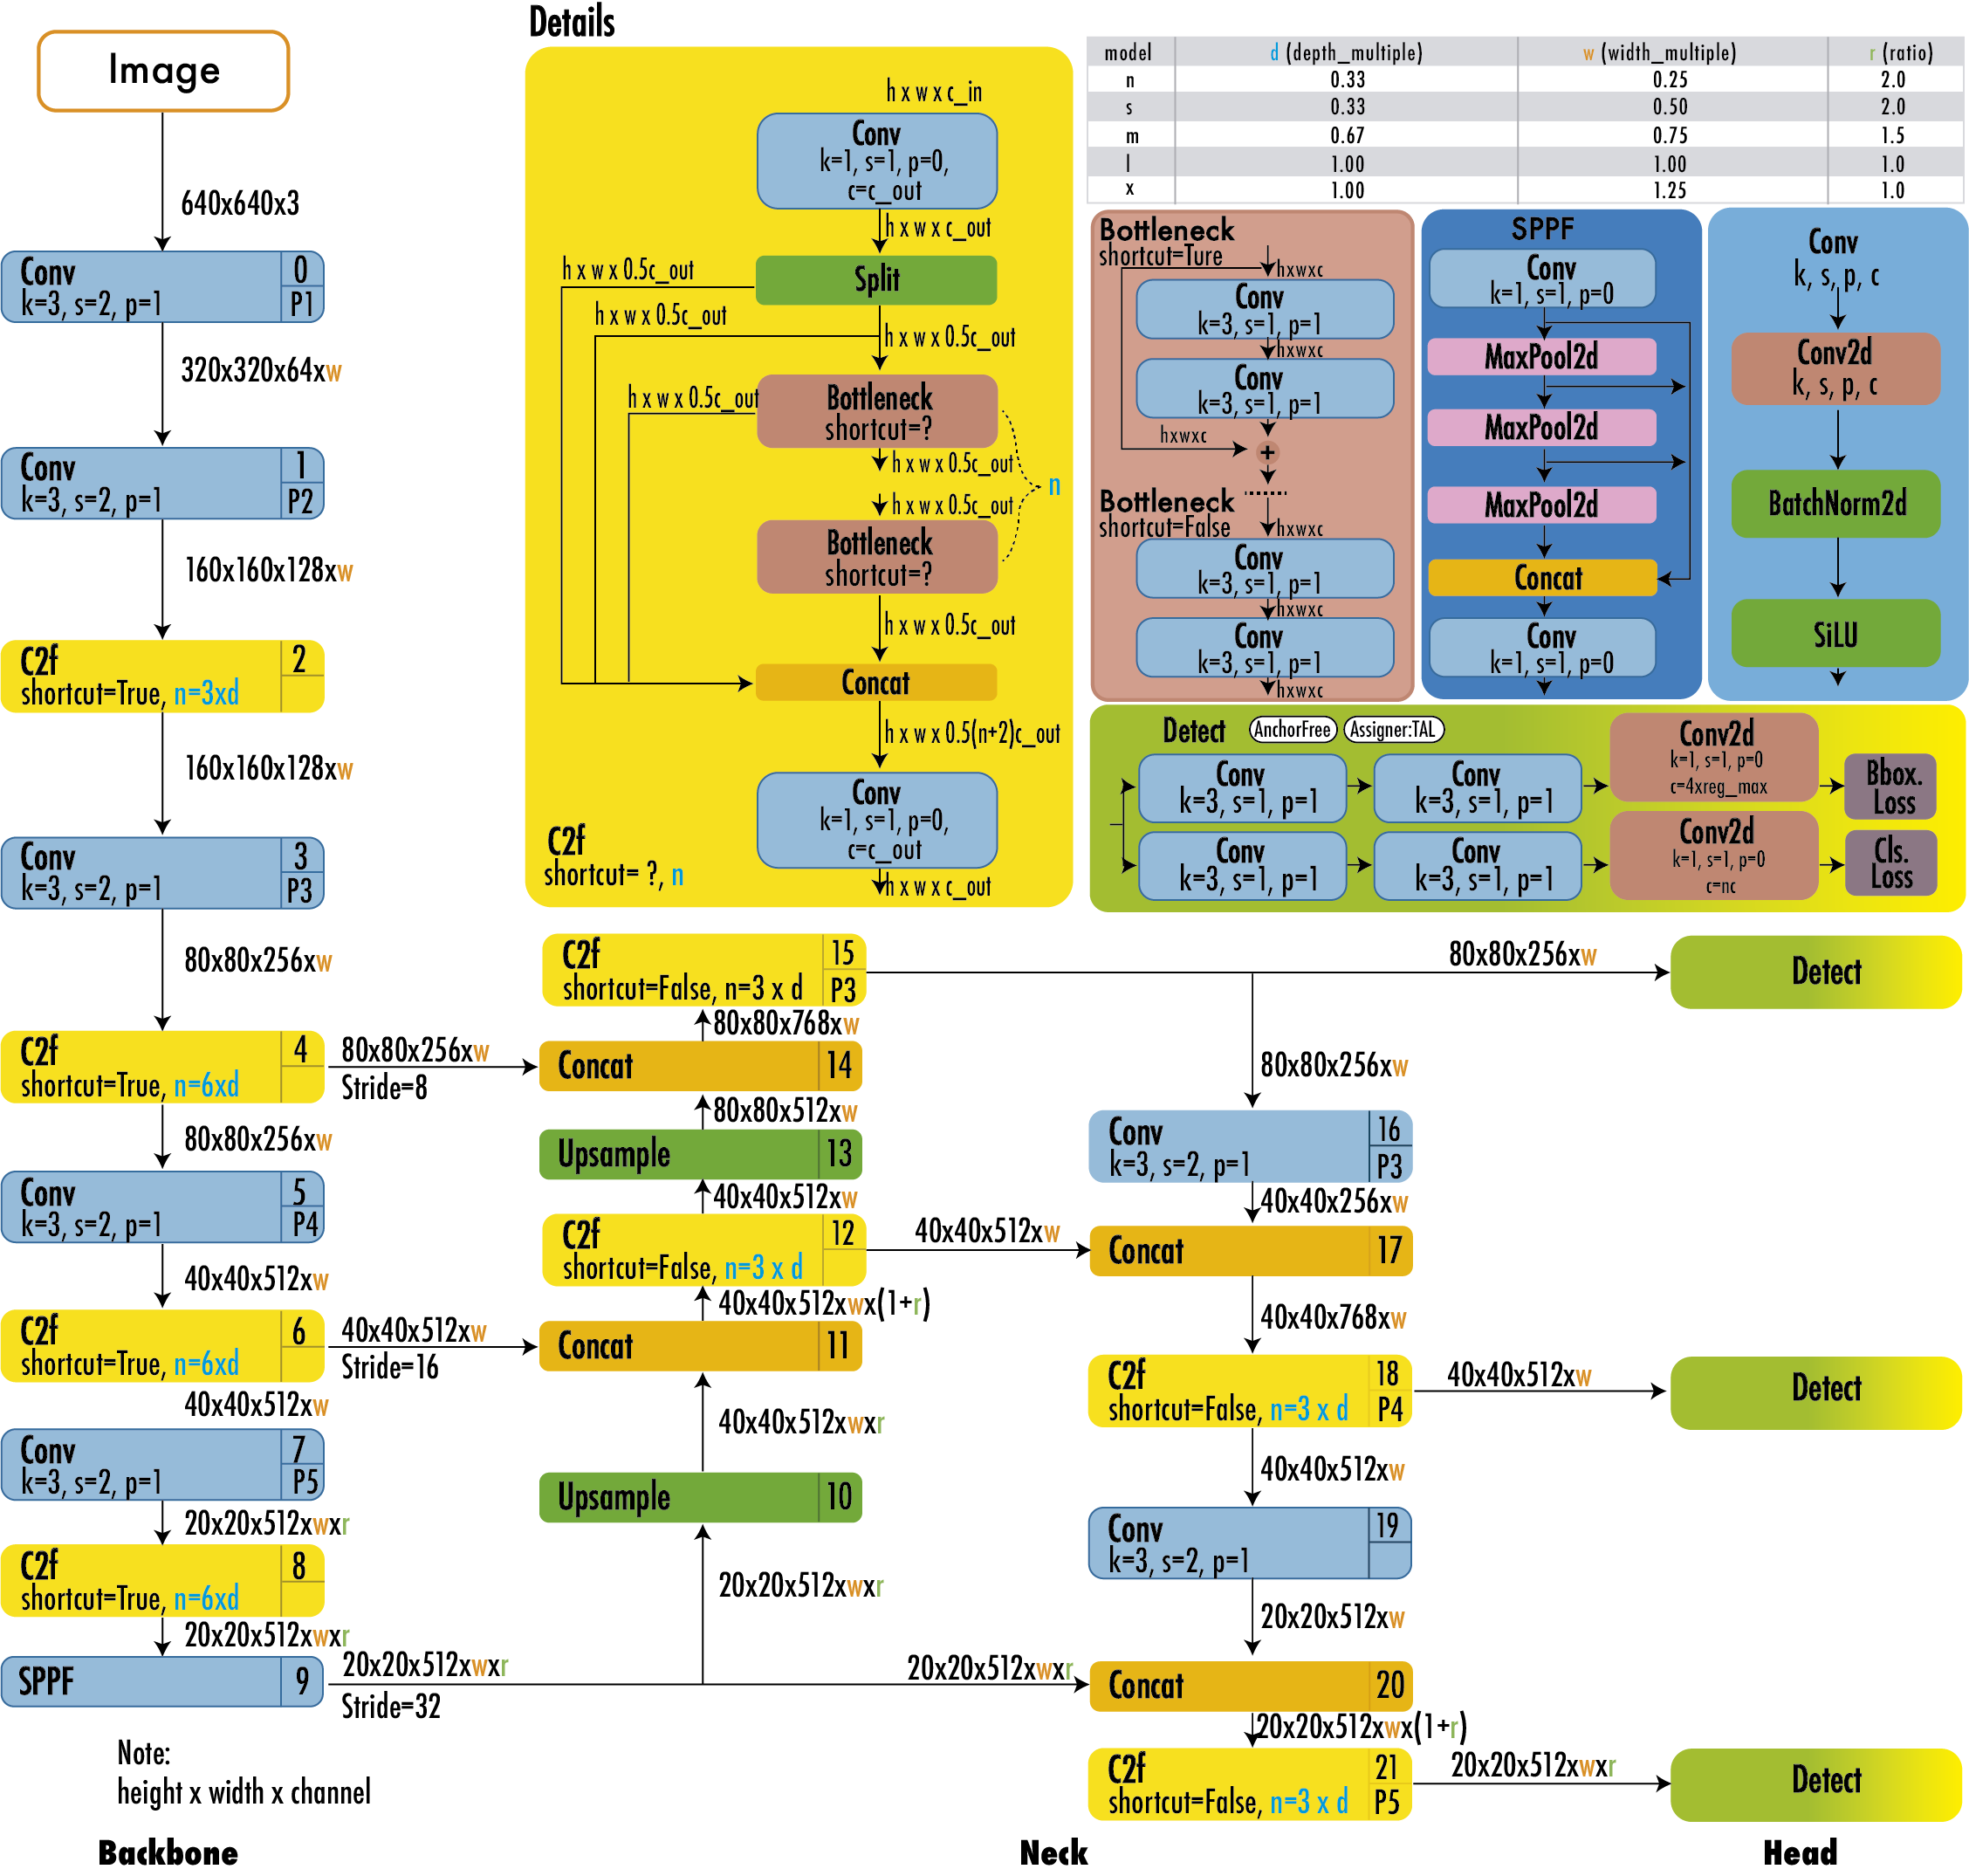
\includegraphics[width=0.85\textwidth]{images/yolov8_architecture.png}
				\caption{YOLOv8 architecture}
				\label{fig:yolov8}
			\end{figure}
		\end{column}
	\end{columns}
\end{frame}

\begin{frame}{Applications}
	\begin{figure}[h]
		\centering
		\includegraphics[width=0.7\textwidth]{images/yolo_apps_.png}
		\caption{Applications on YOLO}
		\label{fig:yolo_apps}
	\end{figure}
\end{frame}

\subsection{Introduction to Combination}
\begin{frame}{Deep Snake}
	\begin{figure}[h]
		\centering
		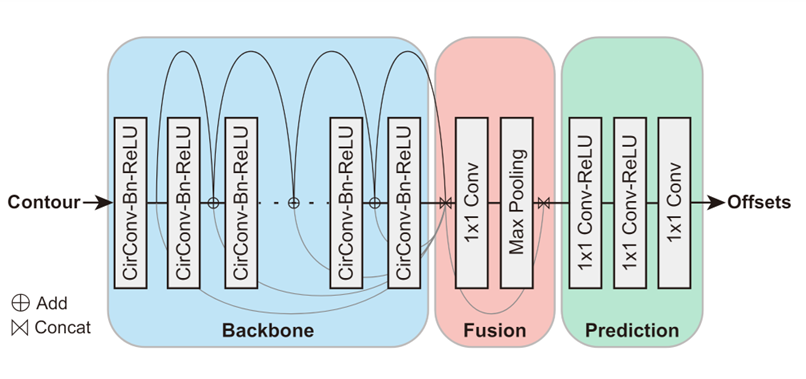
\includegraphics[width=0.7\textwidth]{images/deepsnake_architecture.png}
		\caption{Deep Snake architecture}
		\label{fig:deepsnake_architecture}
	\end{figure}
\end{frame}

